% !TEX root = ../../main.tex

\section{Thermodynamics of adsorption}

As mentioned in the introduction \todo{reference}, adsorption 
is a consequence of intermolecular attraction between the 
material surface and the molecules of the fluid. The sum of 
all interactions accounts for the depth of the potential 
well and therefore for the energy corresponding to the 
process. As this energy is net positive adsorption is an
overall exothermic phenomenon.

However, in order to make the transition from a molecular 
viewpoint to a macroscale bulk fluid representation of 
adsorption, the thermodynamics of the process must be 
clearly defined.


\subsection{Energetic components of adsorption}

From a molecular point of view, we can define the total
interactions taking place during adsorption as a sum of 
several distinct components.

\begin{equation}\label{calo:eqn:interactions}
  \Phi_t = \Phi_{aa} + \Phi_{aa} + \Phi_{aa} + \Phi_{aa}
\end{equation}

The term \(\Phi_{aa}\) is representative of the guest-host
interaction. It can be constant, for a homogeneous surface 
or a function of the occupancy, in the case of a 
heterogeneous surface. The term \(\Phi_{aa}\) is the interaction
between adsorbate molecules. Finally, \(\Phi_{aa}\) is 
a 

Unfortunately, only the total sum of all interactions
is measurable through available methods. Therefore, the 
absolute contribution of each component is unknowable 
through direct methods. However, when used for comparison,
it is likely that the only one contribution has 

\subsection{The Gibbs surface excess approach}

A description of the adsorbed phase can be made through the change
in density or concentration of the fluid starting from the 
adsorbent surface. When represented as such, the density 
has a maxima in the immediate zone close to the surface and then
decreases until attaining the density of the bulk fluid.
However, when defined as such the boundary between the 
adsorbed phase and the bulk phase is difficult to pinpoint.
In some cases, such as adsorption in porous materials, the 
adsorbed phase can be taken as total pore volume, but in 
most cases it is useful to refer to the Gibbs surface 
excess approach of quantifying the amount adsorbed.

This concept describes the adsorbed phase only in terms
of an \textit{excess} from the properties of the bulk phase. 
As long as the volume of the adsorbed layer can be considered 
negligible and the concentration of adsorbate in the bulk 
phase is low, the total amount adsorbed and the surface excess
amount may be considered equal.

\subsection{Enthalpy of adsorption}

From a molecular point of view, we can define the total
interactions taking place during adsorption as a sum of 
several distinct components.

\begin{equation}\label{calo:eqn:interactions}
  \Phi_t = \Phi_{aa} + \Phi_{aa} + \Phi_{aa} + \Phi_{aa}
\end{equation}

The 

Unfortunately, the methods available 

\begin{figure}[htb]
    \centering

    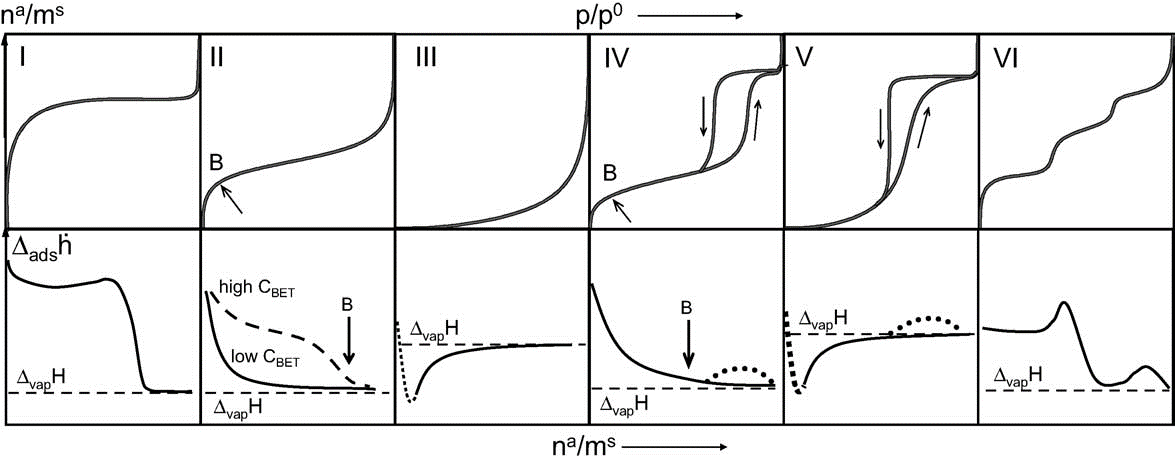
\includegraphics[width=\linewidth]{enthalpy-curves}
    \caption{
      General enthalpy curves corresponding to different 
      IUPAC-defined isotherm 
      types adapted from \citeauthor{llewellynGasAdsorptionMicrocalorimetry2005}%
      \cite{llewellynGasAdsorptionMicrocalorimetry2005}.
    }%
    \label{calo:fig:enthalpy-iupac-iso}

\end{figure}


\subsection{Measuring the enthalpy of adsorption}

Experimentally, two methods are widely used for determining the 
enthalpy of adsorption. The first relies on the applicability of the 
Clausius-Clapeyron equation to two or more isotherms measured 
at different temperatures. The second method relies on a 
direct measurement of the heat produced during adsorption 
using a calorimeter.

There are also ways of determining the enthalpy of adsorption
from computer simulation methods. The accuracy of these methods
depends on the chosen model of interaction with the surface.

\subsubsection{Isosteric heat}

The isosteric heats are calculated from experimental data using the
Clausius-Clapeyron equation as the starting point:

\begin{equation}
    \Big( \frac{\partial \ln P}{\partial T} \Big)_{n_a} = -\frac{\Delta H_{ads}}{R T^2}
\end{equation}

Where \(\Delta H_{ads}\) is the isosteric heat of adsorption.
If it is assumed that the adsorption enthalpy does not vary with 
temperature, the equation can be rearranged to:

\begin{equation}
    \Delta H_{ads} = - R \frac{\partial \ln P}{\partial 1 / T}
\end{equation}

In order to approximate the partial differential, two or more
isotherms are measured at different temperatures. 
Afterwards the isosteric heat of adsorption can be calculated
by using the pressures at which the loading is identical using the 
rearranged equation. By plotting the values of \(\ln P\) against
\(1 / T\) we should obtain a straight line with a slope
of \(- \Delta H_{ads} / R\).

The isosteric heat is sensitive to the differences in pressure between
the two isotherms. If the isotherms measured are too close together, 
the error margin will increase. The method also assumes that enthalpy 
of adsorption does not vary with temperature. If the
variation is large for the system in question, the isosteric
heat calculation will give unrealistic values.

Even with carefully measured experimental data, there are two 
assumptions used in deriving the Clausius-Clapeyron equation: 
an ideal bulk gas phase and a negligible adsorbed phase
molar volume. These have a significant effect on the calculated 
isosteric heats of adsorption, especially at high relative pressures 
and for heavy adsorbates.

\subsubsection{Microcalorimetry}


The enthalpy of adsorption as measured by a calorimeter is a 
sum of all heat contributions during the experiment. They can 
be split into guest-host contributions and host-host contributions.
The guest-host contributions include 

